% !TeX root = RJwrapper.tex
\title{An Algorithm For Spatial Mapping Using a Hexagon Tilegram, With
Application to Australian Maps}
\author{by Stephanie Kobakian, Dianne Cook}

\maketitle

\abstract{%
This algorithm creates a hexagon to represent each of the spatial
polygons provided. It allocates these hexagon in a manner that preserves
the spatial relationship of the areas. It showcases spatial
distributions, by emphasising the small geographical regions that are
often difficult to locate on large geographic maps. Spatial
distributions have been presented on alternative representations of
geography for many years. In modern times, interactivity and animation
have begun to play a larger role, as alternative representations have
been popularised by online news sites, and atlas websites with a focus
on public consumption. Applications are increasingly widespread,
especially in the areas of disease mapping, and election results.
}

% Any extra LaTeX you need in the preamble

\hypertarget{introduction}{%
\subsection{Introduction}\label{introduction}}

Choropleths are the current best practice approach for presenting
geographical data as maps highlight the geographic patterns in
geospatially related statistics (Moore and Carpenter
\protect\hyperlink{ref-SAMGIS}{1999}). The land on the map space is
divided to separate each area, these boundaries are usually
administrative. The areas are filled with colour to represent the value
of the statistic for the area (Tufte \protect\hyperlink{ref-EI}{1990}).

In Australia, government bodies such as the Australian Bureau of
Statistics, or the Australian Electoral Commission hold the
responsibility for the division of areas. These boundaries are often
adjusted as the population in areas increase. Australian people are
increasingly congregating around major cities, the rural areas are often
sparsely populated in comparison to the urban centres. The division of
the population into equal population areas results in dramatically
different square meterage of the geographic areas. This results in an
unequal presentation of the statistic in each area, this can
misrepresent the spatial distributions of the human related statistics
in geographic maps.

Beginning with the geography, cartograms apply a transformation to place
importance on the statistic of interest. They result in a distortion of
the map space to represent differences in the statistic. These displays
rely on the statistic of interest to determine the layout, however for
Australia, many cartograms fail to preserve a recognisable display.
Contiguous cartograms change the shape of an area, preserving
neighbouring relationships. Non-contiguous cartograms maintain the shape
of each area, but lose the connection to neighbours.

Alternative maps shift the focus from land area, to the value of the
statistics in a group of areas. Alternative mapping methods allow
increased understanding of the spatial distribution of a variable across
the population, by fairly representing each administrative area.

Tilegrams are an extension of Dorling cartograms, using one simple shape
to represnt each area. This allows preservation of spatial relationships
and decreases the emphasis from the amount of geographic area. These
maps focus on the relationship between neighbours attempting to preserve
connections, and disregard the unique shapes of the administrative
boundaries.

The \CRANpkg{sugarbag} package provides a new method to implement
hexagon tilegrams. Extending the tilegram to Australian applications
required preserving the spatial relationships. It emphasises the capital
cities as population hubs, and recognises the distances between
locations of populations distributed across the large rural areas.

\hypertarget{algorithm}{%
\section{Algorithm}\label{algorithm}}

This solution operates on a set of \CRANpkg{sf} (Pebesma
\protect\hyperlink{ref-sf}{2019}) polygons.

There are four tasks to create a hexagon tilegram. These steps can be
executed by the main function, \texttt{create\_hexmap}, or can be
applied separately for more flexibility.

\begin{enumerate}
\def\labelenumi{\arabic{enumi}.}
\tightlist
\item
  Create the set of centroids to allocate
\item
  Create the set of hexagons to use
\item
  Allocate each centroid to an available hexagon
\item
  Transform the data for plotting
\end{enumerate}

There are parameters used in the process that can be provided, if they
are not, they will be automatically derived.

\hypertarget{install-sugarbag-package}{%
\subsubsection{Install sugarbag
package}\label{install-sugarbag-package}}

\begin{Schunk}
\begin{Sinput}
# To install sugarbag:
# devtools::install_github("srkobakian/sugarbag")
library(sugarbag)

library(tidyverse)
\end{Sinput}
\begin{Soutput}
#> Registered S3 methods overwritten by 'ggplot2':
#>   method         from 
#>   [.quosures     rlang
#>   c.quosures     rlang
#>   print.quosures rlang
\end{Soutput}
\begin{Soutput}
#> Registered S3 method overwritten by 'rvest':
#>   method            from
#>   read_xml.response xml2
\end{Soutput}
\begin{Soutput}
#> -- Attaching packages --------------------------------------------------- tidyverse 1.2.1 --
\end{Soutput}
\begin{Soutput}
#> v ggplot2 3.1.1       v purrr   0.3.2  
#> v tibble  2.1.1       v dplyr   0.8.0.1
#> v tidyr   0.8.3       v stringr 1.4.0  
#> v readr   1.3.1       v forcats 0.4.0
\end{Soutput}
\begin{Soutput}
#> -- Conflicts ------------------------------------------------------ tidyverse_conflicts() --
#> x dplyr::filter() masks stats::filter()
#> x dplyr::lag()    masks stats::lag()
\end{Soutput}
\end{Schunk}

\hypertarget{parameters}{%
\subsubsection{Parameters}\label{parameters}}

The \texttt{create\_hexmap} function requires several parameters, if
they are not provided, the information will be derived from the polygon
set used. If users already have a grid and set of centroids they may
choose to only use the \texttt{allocate} function.

\textbf{The following must be provided to \texttt{create\_hexmap}:}

\begin{Schunk}

\begin{tabular}{l|l}
\hline
parameter & description\\
\hline
shp & an sf object containing the polygon information\\
\hline
sf\_id & name of a column that distinguishes unique areas\\
\hline
focal\_points & a data frame of reference locations used to allocate hexagons\\
\hline
\end{tabular}

\end{Schunk}

\hypertarget{tasmania-example}{%
\subsubsection{Tasmania example}\label{tasmania-example}}

The polygon set of Local Government Areas (LGA) of Tasmania in 2016 is
provided with the \CRANpkg{sugarbag} package as \texttt{tas\_lga}. A
single column of the data set must be used to identify the unique areas.
In this case, the unique LGA codes associated with each LGA have been
used.

The longitude and latitude centre of the capital cities of Australia are
used to allocate areas around the closest capital city, as this example
uses only the areas in the state of Tasmania, Hobart will be the common
focal point.

\begin{Schunk}
\begin{Sinput}
data(capital_cities)
\end{Sinput}
\end{Schunk}

\textbf{The following parameters will be determined within
\texttt{create\_hexmap} if they are not provided. They are created
throughout the following example:}

\begin{Schunk}

\begin{tabular}{l|l}
\hline
parameter & description\\
\hline
buffer\_dist & a float value for distance in degrees to extend beyond the geometry provided\\
\hline
hex\_size & a float value in degrees for the diameter of the hexagons\\
\hline
hex\_filter & amount of hexagons around centroid to consider for allocation\\
\hline
width & the angle used to filter the grid points around a centroid\\
\hline
\end{tabular}

\end{Schunk}

\hypertarget{create-the-set-of-centroid-points}{%
\subsection{Create the set of centroid
points}\label{create-the-set-of-centroid-points}}

When utilising individual \texttt{sugarbag} functions, we recommend the
following approach: Begin with a set of polygons. The set should be
provided as an \texttt{sf} object, this is a data frame containing a
\texttt{geometry} column.\footnote{The \texttt{read\_shape} function can
  assist in creating this object.} We will use the Local Government
Areas of Tasmania, downloaded from the Australian Bureau of Statistics.

The centroids can be derived from the set of polygons:

\begin{Schunk}
\begin{Sinput}
## Use the create_centroids function to find polygon centroids:
centroids <- create_centroids(shp_sf = tas_lga, sf_id = "LGA_CODE16")
\end{Sinput}
\begin{Soutput}
#> Warning in st_centroid.sf(.): st_centroid assumes attributes are constant
#> over geometries of x
\end{Soutput}
\begin{Soutput}
#> Warning in st_centroid.sfc(st_geometry(x), of_largest_polygon =
#> of_largest_polygon): st_centroid does not give correct centroids for
#> longitude/latitude data
\end{Soutput}
\begin{Sinput}
## Join to data for each area
centroids <- left_join(centroids,
  sf::st_drop_geometry(tas_lga), by = "LGA_CODE16")
\end{Sinput}
\end{Schunk}

\begin{Schunk}
\begin{Sinput}
fort_lga <- fortify_sfc(tas_lga)
polys <- ggplot() + 
  geom_polygon(aes(x = long, y = lat, group = interaction(LGA_NAME16, polygon)), data = fort_lga, fill = "grey", size = 0.3, colour = "lightgrey") +theme_void() + coord_equal()

cents <- ggplot() + 
  geom_polygon(aes(x = long, y = lat, group = interaction(LGA_NAME16, polygon)), data = fort_lga, fill = "grey", size = 0.3, colour = "lightgrey") + geom_point(aes(x=longitude, y = latitude), data = centroids) + theme_void() + coord_equal()

gridExtra::grid.arrange(polys, cents, nrow = 1)
\end{Sinput}
\begin{figure}
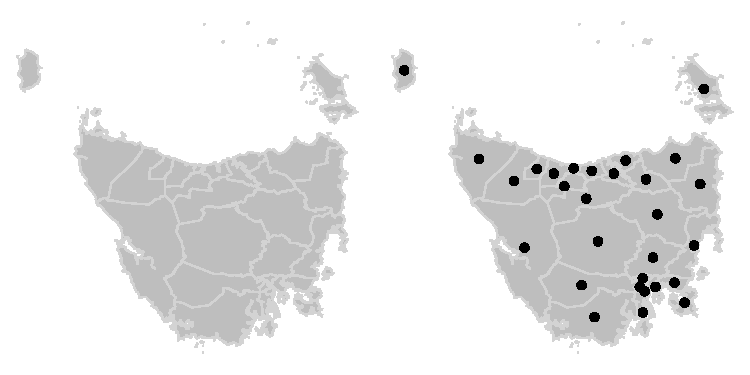
\includegraphics{algorithmRjournal_files/figure-latex/end_cents-1} \caption[Local Government Areas and derived centroids]{Local Government Areas and derived centroids.}\label{fig:end_cents}
\end{figure}
\end{Schunk}

\hypertarget{create-the-hexagon-grid-points}{%
\subsection{Create the hexagon grid
points}\label{create-the-hexagon-grid-points}}

A tilegram allows areas to be allocated to a tellesated set of tiles.
The grid is created to ensure a close point is found, that ensures
tessellation with other previously allocated points.

The grid of possible hexagon centroids can be made using the
\texttt{create\_grid} function. The grid creation requires several
steps. It uses the centroids, the hexagon size and the buffer distance.

\begin{Schunk}
\begin{Sinput}
## create the bounding box from the set of polygon centroids:
bbox <- tibble::tibble(min = c(min(centroids$longitude, na.rm = TRUE), min(centroids$latitude, na.rm = TRUE)),
        max = c(max(centroids$longitude, na.rm = TRUE), max(centroids$latitude, na.rm = TRUE)))

hex_size = 0.3
 
# default size calculation:
#(bbox$max[1] - bbox$min[1])/(bbox$max[2] - bbox$min[2]) / 5
  
buffer_dist <- max((bbox$max[1] - bbox$min[1]), (bbox$max[2] - bbox$min[2]))*0.3
\end{Sinput}
\end{Schunk}

\hypertarget{step-1-expand-the-grid}{%
\subsubsection{Step 1: Expand the grid}\label{step-1-expand-the-grid}}

A sequence is created for longitude columns, and another for latitude
rows.

The sequences begin at the minimum longitude (latitude), minus the
buffer distance. Equally spaced intervals the size of the hexagons are
created up to the maximum longitude (latitude), plus the buffer
distance.

An individual point is created from all intersections of the longitude
columns and latitude row sequences.

\begin{Schunk}
\begin{Sinput}
grid <- tibble::as_tibble(
  expand.grid(
    hex_long = seq(bbox$min[1] - buffer_dist, # minimum
      bbox$max[1] + buffer_dist, # maximum
      hex_size), # distance between hexagons
    hex_lat = seq(bbox$min[2] - buffer_dist, # minimum
      bbox$max[2] + buffer_dist, # maximum
      hex_size))) # distance between hexagons
\end{Sinput}
\end{Schunk}

\begin{Schunk}
\begin{Sinput}
grid1 <- ggplot() + geom_polygon(aes(x = long, y = lat, group = interaction(LGA_NAME16, polygon)), data = fort_lga, fill = "grey", size = 0.3, colour = "lightgrey") + geom_point(aes(x=longitude, y = latitude), data= centroids, colour = "#b2df8a") + theme_void() + coord_equal() +
  geom_point(aes(x = hex_long, y = hex_lat), colour = "#1f78b4", data = grid, size = 0.75) 
\end{Sinput}
\end{Schunk}

A square grid will not facilitate tessellated hexagons. Every second
latitude row of points will be shifted right by half of the hexagon
size.

\begin{Schunk}
\begin{Sinput}
# Find every second latitude
shift_lat <- grid %>% dplyr::select(hex_lat) %>%
    dplyr::distinct() %>%
    dplyr::filter(dplyr::row_number() %% 2 == 1) %>% unlist()

# Shift the longitude of every second latitude to the right to make hex structure
grid <- grid %>%
    dplyr::mutate(hex_long = ifelse(hex_lat %in% shift_lat, hex_long,
        hex_long + (hex_size / 2))) %>%
    dplyr::mutate(id=1:NROW(.)) %>%
    dplyr::mutate(assigned=FALSE)
\end{Sinput}
\end{Schunk}

\begin{Schunk}
\begin{Sinput}
grid2 <- ggplot() + geom_polygon(aes(x = long, y = lat, group = interaction(LGA_NAME16, polygon)), data = fort_lga, fill = "grey", size = 0.3, colour = "lightgrey") + geom_point(aes(x=longitude, y = latitude), data = centroids, colour = "#b2df8a") + theme_void() + coord_equal() +
  geom_point(aes(x = hex_long, y = hex_lat), colour = "#1f78b4", data = grid, size = 0.75) 
\end{Sinput}
\end{Schunk}

Each point is now given an ID.

\begin{Schunk}
\begin{Sinput}
full_grid <- grid <- grid %>%
    mutate(hex_long_int = dense_rank(hex_long)-1,
        hex_lat_int = dense_rank(hex_lat)-1)
\end{Sinput}
\end{Schunk}

\begin{Schunk}
\begin{Sinput}
gridExtra::grid.arrange(grid1, grid2, nrow = 1)
\end{Sinput}
\begin{figure}
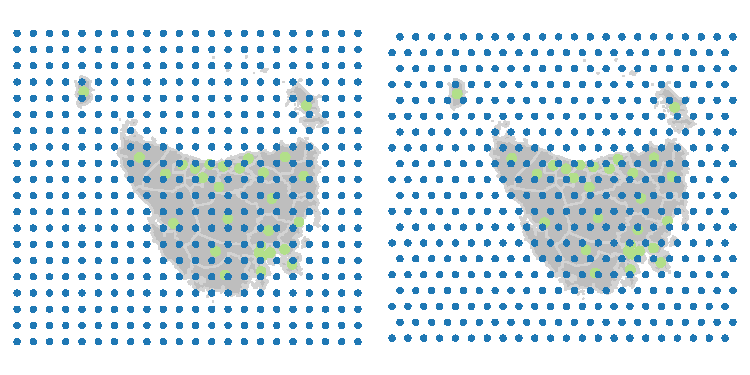
\includegraphics{algorithmRjournal_files/figure-latex/unnamed-chunk-2-1} \caption[Grid points to create a tilegram]{Grid points to create a tilegram.}\label{fig:unnamed-chunk-2}
\end{figure}
\end{Schunk}

\hypertarget{step-2-rolling-windows}{%
\subsubsection{Step 2: Rolling windows}\label{step-2-rolling-windows}}

Not all of the grid points will be used, especially if islands result in
a large grid space. To filter the grid for appropriate points for
allocation, the \texttt{create\_buffer} function is called from
\texttt{create\_grid}. It finds the grid points needed to best capture
the set of centroids.

\begin{Schunk}
\begin{Sinput}
nlong <- length(unique(grid$hex_long))
nlat <- length(unique(grid$hex_lat))

centroids <- centroids %>%
  mutate(long_int = round((longitude-min(grid$hex_long))/(max(grid$hex_long)-min(grid$hex_long))*nlong, 0),
          lat_int = round((latitude-min(grid$hex_lat))/(max(grid$hex_lat)-min(grid$hex_lat))*nlat, 0))
\end{Sinput}
\end{Schunk}

The rows and columns are divided into 20 groups. The amount of rows in
each latitude group and the amount of columns in each longitude group
are then used as the width of rolling windows. This will tailor the
available grid points to the most likely to be used point. It also helps
reduce amount of time taken, as it decreases the amount of points
considered.

The first rolling window function finds the minimum and maximum centroid
values for the sliding groups of longitude columns and the groups of
latitude rows.

The second rolling window function finds the average of the rolling
centroid values minimum and maximum, for the longitude columns and
latitude rows.

\hypertarget{step-3-filtering-the-grid}{%
\subsubsection{Step 3: Filtering the
grid}\label{step-3-filtering-the-grid}}

Only the grid points between the rolling average of the minimum and
maximum centroid values are kept, for each row and column of the grid.

\begin{Schunk}

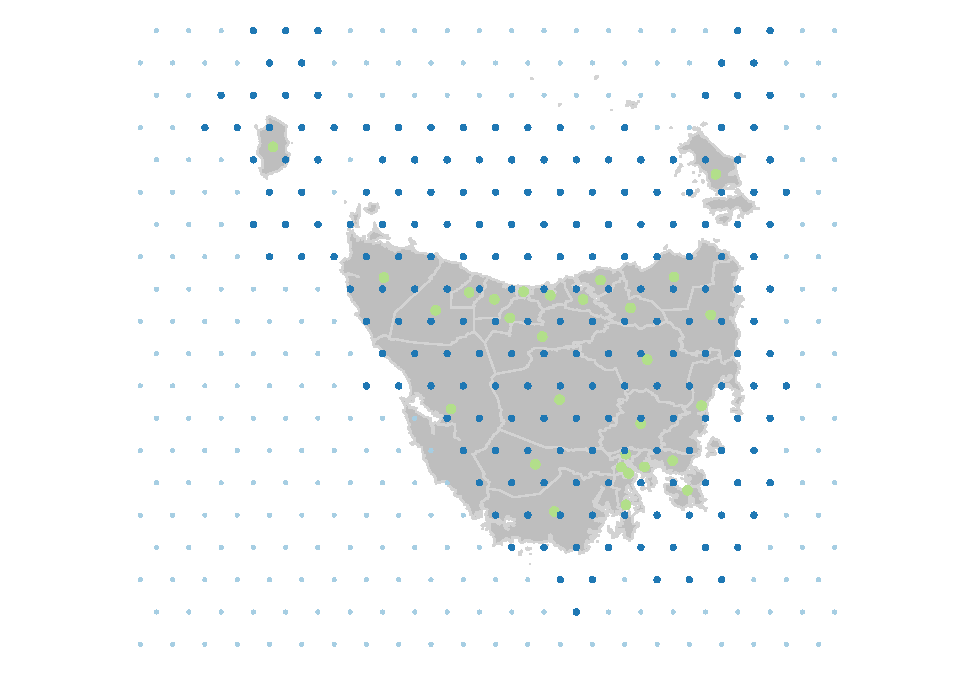
\includegraphics{algorithmRjournal_files/figure-latex/filter_grid-1} \end{Schunk}

\hypertarget{centroid-to-focal-point-distance}{%
\subsection{Centroid to focal point
distance}\label{centroid-to-focal-point-distance}}

\begin{Schunk}
\begin{Sinput}
# Split the centroid data set
centroids <- centroids %>% 
  nest(longitude, latitude) %>% 
  mutate(closest = map(data, closest_focal_point, focal_points = capital_cities %>% filter(points == "Hobart"))) %>% 
  unnest(data, closest) %>% 
  arrange(focal_distance)
\end{Sinput}
\end{Schunk}

For each polygon centroid in the set, the distance to each of the focal
points provided is recorded. The closest focal point name, the distance
to the polygon centroid, and the angle from focal point to polygon
centroid will be added to the polygon's row, in the polygon data set. To
minimise time taken for this step, only Tasmania's capital city Hobart
has been provided.

The distance between the polygon centroid and it's closest focal point
data set is used to order the data set for allocation. The points are
arranged in ascending order, from the centroid closest to any of the
focal points, to the furthest.

\hypertarget{allocate-each-centroids-to-a-hexagon-grid-point}{%
\subsection{Allocate each centroids to a hexagon grid
point}\label{allocate-each-centroids-to-a-hexagon-grid-point}}

The distance around a centroid to consider for possible hexagon
locations is determined by the hex\_filter. It multiplies the amount
given by hex\_filter, by the size of the hexagons to find the distance.

\begin{Schunk}
\begin{Sinput}
hexmap_allocation <- allocate(
  centroids = centroids,
  sf_id = "LGA_CODE16",
  hex_grid = grid,
  hex_size = 0.2, # same size used in create_grid
  hex_filter = 10,
  width = 35,
  focal_points = capital_cities,
  verbose = TRUE
)
\end{Sinput}
\end{Schunk}

Allocation of all centroids can now take place using the set of polygon
centroids and the hexagon map grid. For each polygon centroid, only the
hexagon grid points that have not yet been used can be considered.
Allocate each centroid, beginning with the closest centroid to a focal
point. This will preserve spatial relationship with the capital, as the
inner areas will be allowed closest to the capital, and the areas that
are further will be accommodated after.

\begin{Schunk}
\begin{Sinput}
s_centroids <- centroids %>% arrange(focal_distance)

s_centroids <- split(s_centroids, s_centroids[["focal_distance"]])
        
# Set up allocation data frame
centroid_allocation <- NULL
\end{Sinput}
\end{Schunk}

The filter parameter is used to subset possible grid points to only
those surrounding the polygon centroid within the filter distance,
smaller distance will increase speed, but can decrease accuracy.

\begin{Schunk}
\begin{Sinput}
hex_filter = 10
width = 35
# keep value to reset expanded distances
expand_dist <- hex_filter
\end{Sinput}
\end{Schunk}

The following example considers one of the Local Government Areas. These
steps are repeated for each polygon.

\hypertarget{step-1-filter-the-grid-for-unassigned-hexagon-points}{%
\subsubsection{Step 1: Filter the grid for unassigned hexagon
points}\label{step-1-filter-the-grid-for-unassigned-hexagon-points}}

Keep only the available hexagon points, this will prevent multiple areas
being allocated to the same hexagon.

\begin{Schunk}
\begin{Sinput}
# filter for only the available hex grid points
hex_grid <- grid %>% filter(!assigned)
\end{Sinput}
\end{Schunk}

\hypertarget{step-2-filter-the-grid-points-for-those-closest-to-the-centroid}{%
\subsubsection{Step 2: Filter the grid points for those closest to the
centroid}\label{step-2-filter-the-grid-points-for-those-closest-to-the-centroid}}

This will allow only the closest points, that are not assigned, to be
considered.

\begin{Schunk}
\begin{Sinput}
filter_dist <- hex_filter*hex_size

# filter grid for avaiable points
centroid1 <- centroids %>% head(1)

flong <- centroid1$longitude
flat <- centroid1$latitude

hex_grid <- hex_grid %>% ungroup() %>%
        filter(flat - filter_dist < hex_lat & hex_lat < flat + filter_dist) %>%
        filter(flong - filter_dist < hex_long & hex_long < flong + filter_dist)
\end{Sinput}
\end{Schunk}

Create a box of possible hexagon locations around the centroid. The
bottom of the box will not be square as the buffer has already removed
unnecessary points from over the ocean.

The algorithm removes the outer corners of the square, creating a circle
of points, by only keeping points within a certain radius around the
original centroid location.

\begin{Schunk}
\begin{Sinput}
    hex_grid <- hex_grid %>%
        rowwise %>%
        mutate(
        hex_lat_c = hex_lat - flat,
        hex_long_c = hex_long - flong) %>%
        mutate(hyp = ((hex_lat_c^2) + (hex_long_c^2))^(1/2))


        f_angle <- centroid1 %>%
            mutate(atan = atan2(latitude-latitude1,longitude-longitude1),
                angle = (atan*180/pi),
                pangle = ifelse(angle<0, angle +360, angle)) %>% pull()


        hex_grid <- hex_grid %>%
            # create circle of radius: hex_filter
            filter(hyp < filter_dist) %>%
            mutate(
                # geosphere takes a long time
                angle = f_angle,
                angle_plus = (angle + width)%%360,
                angle_minus = (angle - width)%%360,
                atan = atan2(hex_lat_c, hex_long_c),
                hex_angle = (atan*180/pi),
                hex_angle = ifelse(hex_angle<0, hex_angle +360, hex_angle))
\end{Sinput}
\end{Schunk}

\begin{Schunk}
\begin{Sinput}
gridExtra::grid.arrange(buff1, buff2, nrow=1)
\end{Sinput}

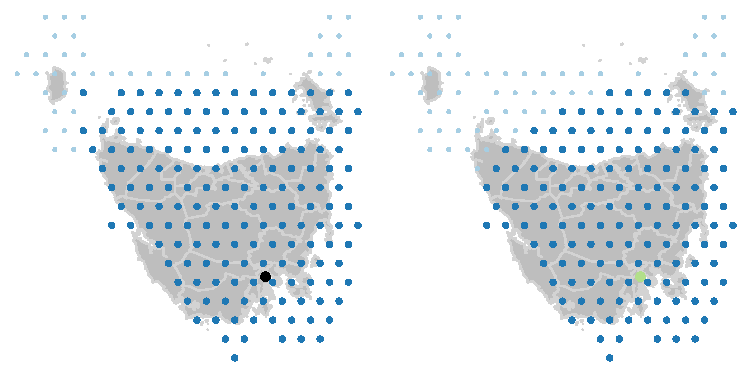
\includegraphics{algorithmRjournal_files/figure-latex/buffers-1} \end{Schunk}

The width parameter is now used. Of the remaining points, a slice is
taken. This uses the angle from the closest capital city, to the current
centroid. If it is not the closest to the capital there may have been
points available that were taken by closer centroids. This allows the
spatial relationship to be preserved, even when it gets allocated to a
hexagon that is further from the city centre. This angle begins at 30
degrees by default, and may increase if necessary.

If no available hexagon grid point is found within the original filter
distance and angle, the distance is expanded, only when a maximum
distance is reached will the angle expand to accommodate more possible
grid points.

The allocation is returned and combined with the data relating to each
polygon.

\begin{Schunk}
\begin{Sinput}
# Filter for angle within circle

        if (hex_grid$angle_minus[1] < hex_grid$angle_plus[1]) {
            hex_grid <- hex_grid %>%
                # create slice of 60 degrees from centroid
                filter(angle_minus < hex_angle & hex_angle < angle_plus)
        } else {
            hex_grid <- hex_grid %>%
                # create slice of 60 degrees from centroid
                filter(hex_angle < angle_plus | angle_minus > hex_angle)
        }
\end{Sinput}
\end{Schunk}

\begin{Schunk}
\begin{Sinput}
ggplot() + geom_polygon(aes(x = long, y = lat, group = interaction(LGA_NAME16, polygon)), data = fort_lga, fill = "grey", size = 0.3, colour = "lightgrey") + theme_void() + coord_equal() +
  geom_point(aes(x = hex_long, y = hex_lat), colour = "#a6cee3", data = grid, size = 0.25) +
  geom_point(aes(x = hex_long, y = hex_lat), colour = "#1f78b4", data = hex_grid, size = 0.75) + 
  geom_point(aes(x=longitude, y = latitude), data = centroid1, colour = "#b2df8a", size = 0.8) 
\end{Sinput}

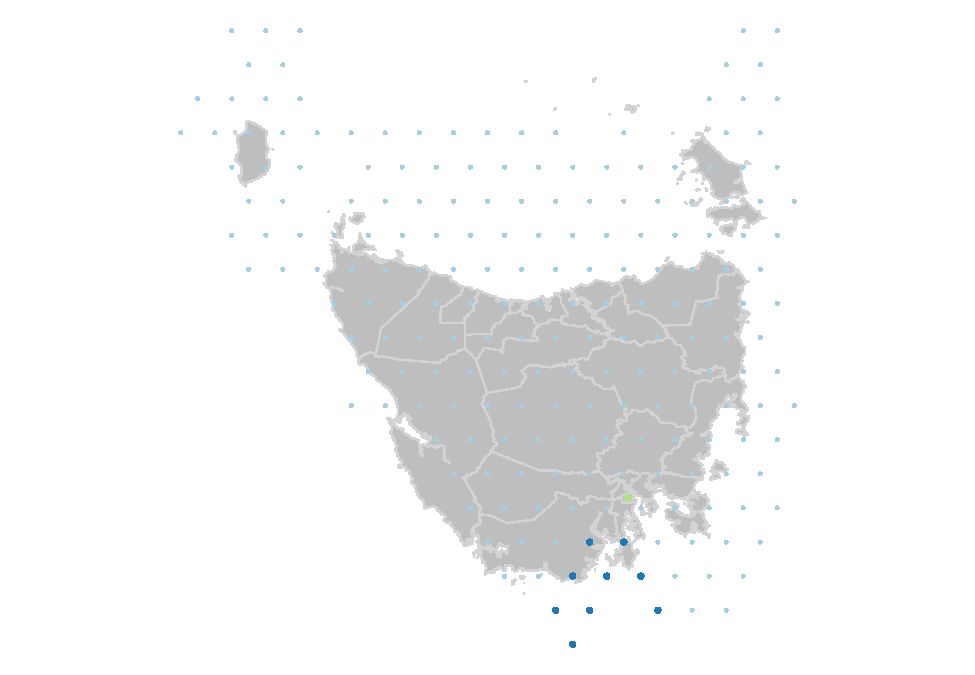
\includegraphics{algorithmRjournal_files/figure-latex/plot_slice-1} \end{Schunk}

This area was the very closest to the Hobart central point ( coloured
pink) provided in the capital cities data set, it gets a hexagon point
(coloured blue) extremely close to it's centroid (coloured green).

\begin{Schunk}
\begin{Sinput}
# Choose first available point
cent <- centroid1 %>% dplyr::rename(focal_point = points, focal_dist = focal_distance, focal_angle = angle)

# Filter should give one hex point
hex <- hex_grid %>% 
  ungroup %>% 
  filter(hyp == min(hyp)) %>%
  select(hex_long, hex_lat, hex_id = id)

# Update grid to show this centroid as assigned
hex_grid[which(hex_grid$id == hex$hex_id),]$assigned <- TRUE

# Add to table of allocated centroids
centroid_allocation <- bind_rows(centroid_allocation, dplyr::bind_cols(cent, hex)) %>% as_tibble()
\end{Sinput}
\end{Schunk}

\begin{Schunk}
\begin{Sinput}
hex_points_df <- centroid_allocation %>% 
  fortify_hexagon(hex_size = hex_size,
  sf_id = "LGA_CODE16")
\end{Sinput}
\end{Schunk}

\begin{Schunk}
\begin{Sinput}
ggplot() + 
  geom_polygon(aes(x = long, y = lat, group = interaction(LGA_NAME16, polygon)), data = fort_lga %>% filter(LGA_CODE16=="62810"), fill = "grey", size = 0.3, colour = "lightgrey") +
  geom_point(aes(x = hex_long, y = hex_lat), colour = "#1f78b4", data = hex_grid, size = 0.75) + 
  geom_point(aes(x=longitude1, y = latitude1), data = centroid1, colour = "#fb9a99", size = 1) + 
  geom_point(aes(x=longitude, y = latitude), data = centroid1, colour = "#b2df8a", size = 0.8) + 
  theme_void() +
  coord_equal()
\end{Sinput}

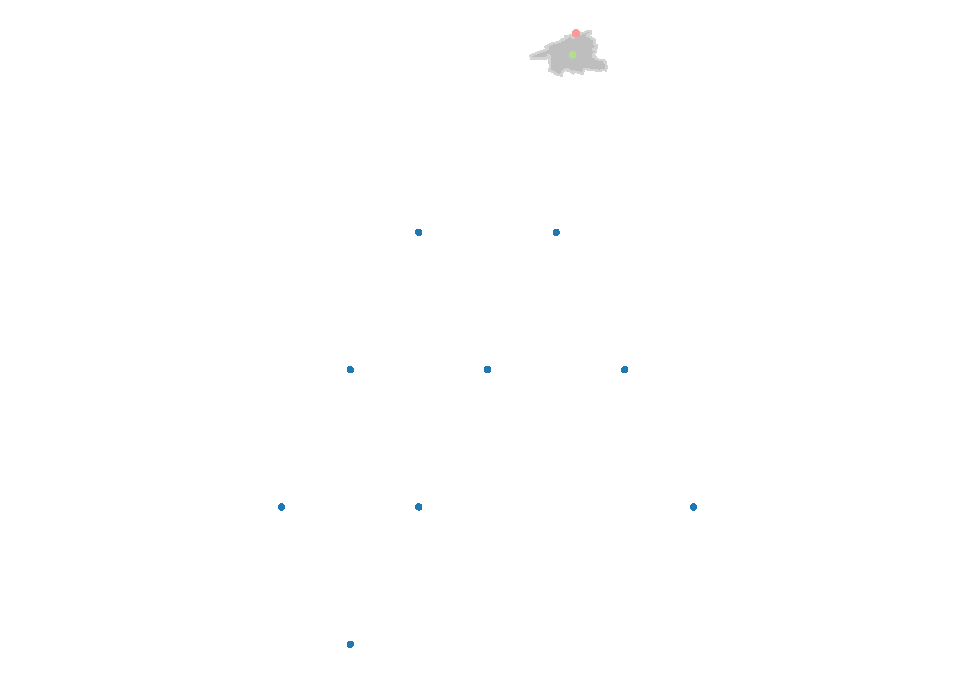
\includegraphics{algorithmRjournal_files/figure-latex/plot_allocated-1} \end{Schunk}

The following code creates a map for all the Local Government Areas in
Tasmania:

\begin{Schunk}
\begin{Sinput}
# Create centroids set
centroids <- create_centroids(tas_lga, "LGA_CODE16")
\end{Sinput}
\begin{Soutput}
#> Warning in st_centroid.sf(.): st_centroid assumes attributes are constant
#> over geometries of x
\end{Soutput}
\begin{Soutput}
#> Warning in st_centroid.sfc(st_geometry(x), of_largest_polygon =
#> of_largest_polygon): st_centroid does not give correct centroids for
#> longitude/latitude data
\end{Soutput}
\begin{Sinput}
# Create hexagon location grid
grid <- create_grid(centroids = centroids,
    hex_size = 0.3,
    buffer_dist = 1.2)
# Allocate polygon centroids to hexagon grid points
hex_allocated <- allocate(
  centroids = centroids,
  hex_grid = grid,
  sf_id = "LGA_CODE16",
  # same column used in create_centroids
  hex_size = 0.3,
  # same size used in create_grid
  hex_filter = 10,
  focal_points = capital_cities %>% filter(points == "Hobart"),
  width = 35,
  verbose = FALSE
)
\end{Sinput}
\begin{Soutput}
#> Allocating centroids, in order of distance to closest focal point.
\end{Soutput}
\end{Schunk}

\begin{Schunk}
\begin{Sinput}
h1 <- hex_allocated %>%
  fortify_hexagon(hex_size = 0.3, 
  sf_id = "LGA_CODE16") %>% 
  left_join(., tas_lga)
\end{Sinput}
\begin{Soutput}
#> Joining, by = "LGA_CODE16"
\end{Soutput}
\begin{Soutput}
#> Warning: Column `LGA_CODE16` joining character vector and factor, coercing
#> into character vector
\end{Soutput}
\begin{Sinput}
p1 <- fortify_sfc(tas_lga)
end_hex <- ggplot() +
  geom_polygon(data = p1, aes(x=long, lat, group = interaction(LGA_NAME16, polygon)), fill = "grey", size = 0.3, colour = "lightgrey") +
  geom_polygon(data = h1, aes(x=long, lat, group = LGA_CODE16)) + theme_void() + coord_equal()

gridExtra::grid.arrange(cents, end_hex, nrow = 1)
\end{Sinput}

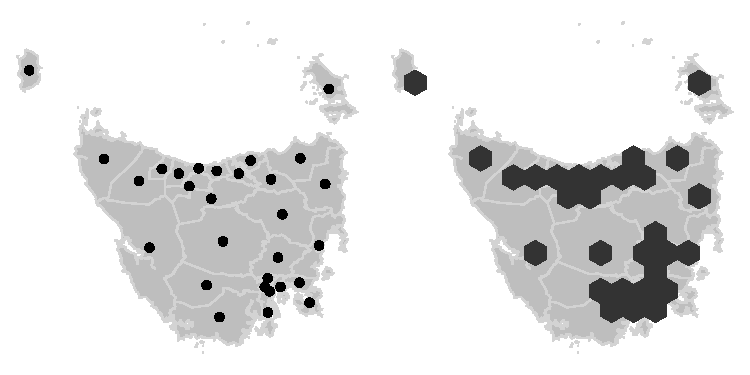
\includegraphics{algorithmRjournal_files/figure-latex/plot_final-1} \end{Schunk}

\hypertarget{summary}{%
\subsection{Summary}\label{summary}}

It is possible to use alternative maps to communicate spatial
distributions. Current methods do not always work for Australia due to
the large gaps between densely populated capital cities.

\hypertarget{code}{%
\subsection{Code}\label{code}}

This map algorithm is found in the \texttt{sugarbag} package, currently
available on github: \url{https://github.com/srkobakian/sugarbag}

R Core Team (\protect\hyperlink{ref-R}{2012})

\bibliography{algorithmbib}

\hypertarget{refs}{}
\leavevmode\hypertarget{ref-SAMGIS}{}%
Moore, Dale A., and Tim E. Carpenter. 1999. ``Spatial Analytical Methods
and Geographic Information Systems: Use in Health Research and
Epidemiology.'' \emph{Epidemiologic Reviews} 21 (2): 143--61.
\url{https://doi.org/10.1093/oxfordjournals.epirev.a017993}.

\leavevmode\hypertarget{ref-sf}{}%
Pebesma, Edzer. 2019. \emph{Sf: Simple Features for R}.
\url{https://CRAN.R-project.org/package=sf}.

\leavevmode\hypertarget{ref-R}{}%
R Core Team. 2012. \emph{R: A Language and Environment for Statistical
Computing}. Vienna, Austria: R Foundation for Statistical Computing.
\url{http://www.R-project.org/}.

\leavevmode\hypertarget{ref-EI}{}%
Tufte, Edward R. 1990. \emph{Envisioning Information}. Graphics Press.

\bibliography{RJreferences.bib}

\address{%
Stephanie Kobakian\\
Queensland University of Technology\\
\\
}
\href{mailto:stephanie.kobakian@monash.edu}{\nolinkurl{stephanie.kobakian@monash.edu}}

\address{%
Dianne Cook\\
Monash University\\
\\
}
\href{mailto:dicook@monash.edu}{\nolinkurl{dicook@monash.edu}}

